\documentclass[10pt]{article}

\usepackage{amsmath}
\usepackage{fullpage}
\usepackage{array}
\usepackage{graphicx}
\usepackage{gensymb}
\usepackage{booktabs}
\usepackage{gensymb}
\usepackage{graphicx}

\graphicspath{ {../Images/} }

\date{2014-6-22}
\pagestyle{empty}
\setlength{\parindent}{0pt}

\begin{document}
\begin{center}
\begin{Large}\textbf{Physical Science 303 - Activity}\end{Large} \\
\smallskip
%\begin{large} Acceleration \end{large}
\end{center}
%%%%%%%

\section{Work-Energy}
\subsection{Review}
We first review the notions of kinetic energy and work.  The energy associated with the motion of the particle (moving with non-relativistic speed) is the kinetic energy.  It is given by
\begin{equation}
  KE = \frac{1}{2}mv^2
\end{equation}
where $m$ is the mass and $v$ is the speed of the particle.  

The work done by a force $\vec{F}$ which produces the displacement $\vec{d}$ is given by the scalar product
\begin{equation}
  W=\vec{F}.\vec{d}
\end{equation}

Work and energy have same units!  
 
Work-energy theorem says that \emph{work done by all the forces is total change in KE}.  Symbolically
\begin{equation}
  W_{\text{all}} = \Delta KE_{\text{total}}
\end{equation}

\subsection{Activity}
\begin{enumerate}
\item \textbf{Required Box}: Box 1
\item \textbf{Required Items}: Spring (Every color will work! Try Red for the start.), hanging rod, thread, 1N, 2N and 3N weights and ruler.
\end{enumerate}
\begin{enumerate}
\item Measure the unstreched length of the spring. Length ($l_0$):\underline{\hspace{5cm}}cm
\item Prepare the setup as shown.  \emph{Make sure to provide the support such that the spring is unstretched}
\begin{figure}[h]
\label{springunhand}
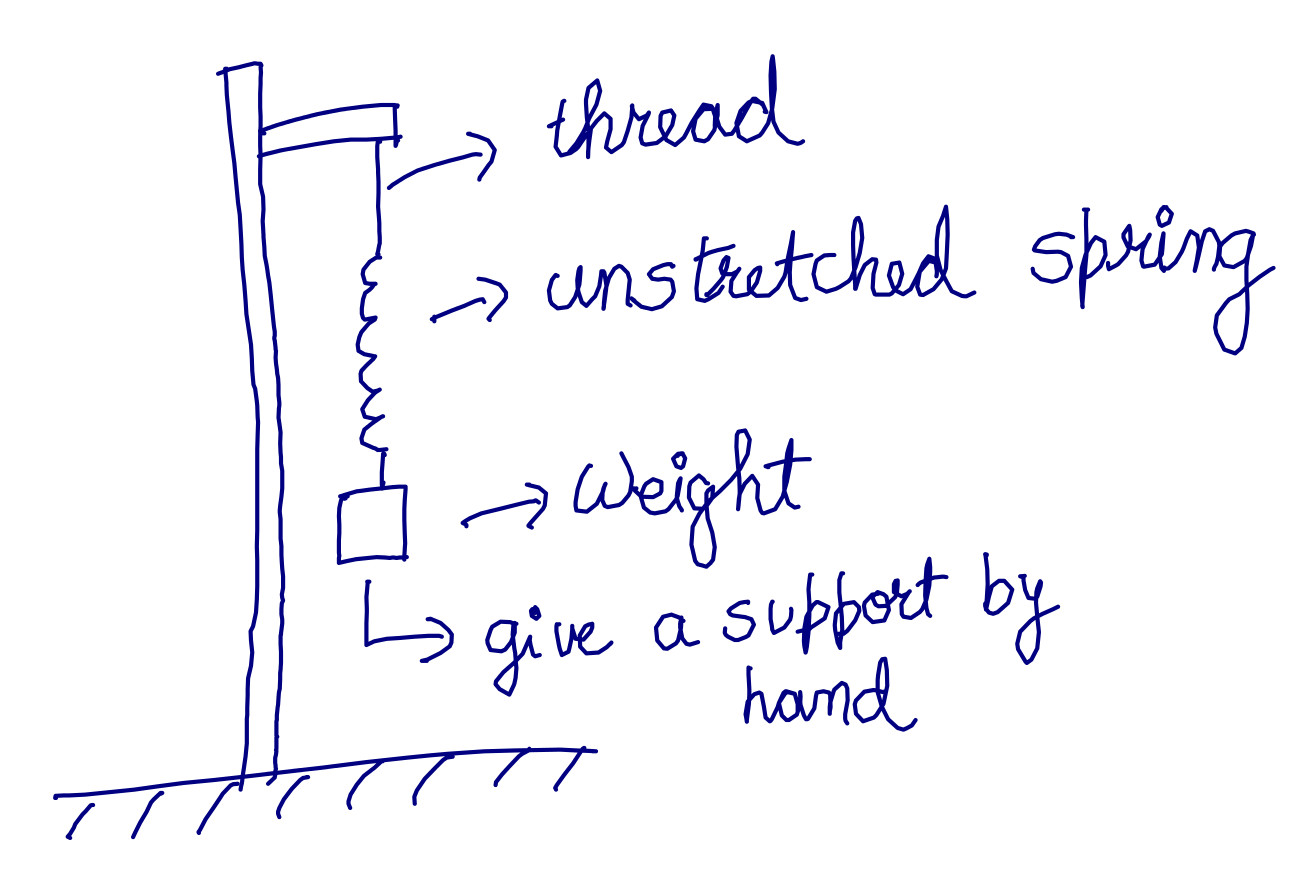
\includegraphics[scale=.5]{springunhand}
\centering
\caption{Setup: Unstretched spring}
\end{figure}
\item Now remove the support and let gravity work on the weight.  Observe the motion of the weight and once it reaches the \emph{farthest} point (actually, as you can imagine, it will oscillate up and down), hold it using your hand (it is little tricky but should be doable after 2-3 attempts) as shown in the figure \ref{springsthand}. 
\begin{figure}[h]
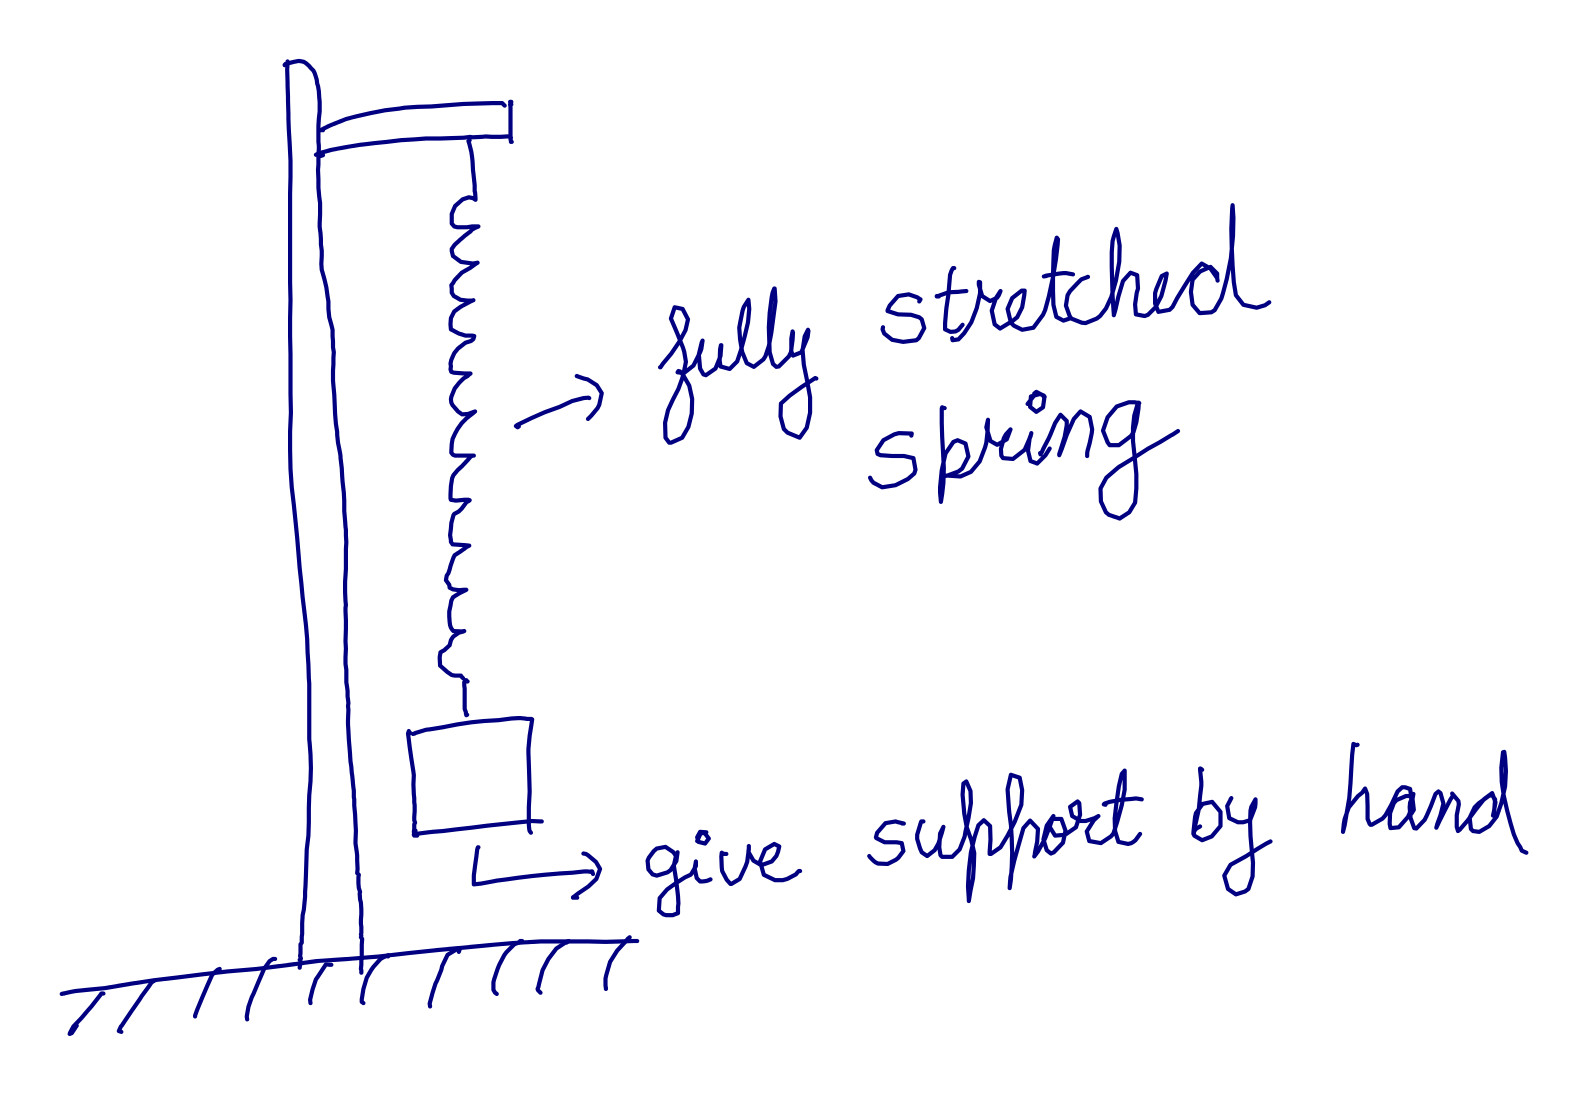
\includegraphics[scale=.5]{springsthand}
\centering
\caption{Setup: Fully stretched spring}
\label{springsthand}
\end{figure}
Measure the \textbf{fully stretched} length of the spring.  Repeat the process for all the available weights and fill the table below.   
\end{enumerate}
\begin{center}
 \begin{tabular}{||c c c||} 
 \hline
 Weight $W_n$ (N) & Fully stretched length $l$ (cm) & difference $\delta x = l-l_0$ (cm)\\ [0.5ex] 
 \hline\hline
 1 &  & \\ 
 \hline
 2 &  &\\
\hline
 3 & &\\
\hline
\end{tabular}
\end{center}

\subsection{Theoretical Analysis}
In this section we aim to conduct a theoretical study based on the experiment
\begin{enumerate}
\item Compute the fraction $\frac{\delta x}{W_n}$ for all the three weights and write them down below (with proper units)
\vspace{100px}
  \begin{enumerate}
  \item $f_1$:\underline{\hspace{5cm}}
  \item $f_2$:\underline{\hspace{5cm}}
  \item $f_3$:\underline{\hspace{5cm}}  
  \end{enumerate}
\item What do you observe?  Are $f_1$, $f_2$ and $f_3$ almost equal? 
\vspace{50px}
\item If yes, then (theoretically speaking!) let $f_1=f_2=f_3=\frac{1}{\kappa}$, $W_n=mg$ and $\delta x = d$.  Thus we have 
  \begin{equation}
    \begin{split}
      \frac{1}{\kappa} &= \frac{d}{mg}\\
      mg &= \kappa d
    \end{split}
  \end{equation}
and now multiply $d$ on both the sides to get 
\begin{equation}
\label{gravwork}
mgd = \kappa d^2 
\end{equation}
\item Do you recognize the LHS of the above equation?  What does it correspond to physically?
\vspace{50px}
\item The RHS contains two variables.  $d$ represents the extension produced in the \emph{spring}.  $\kappa$ should represent the property of \underline{\hspace{5cm}} (spring or the hanging mass?).
\item What are the units of $\kappa d^2$?  Which physical quantities do they correspond to?
\vspace{50px}
\begin{enumerate}
\item Physical quantity 1 \underline{\hspace{5cm}}
\item Physical quantity 2 \underline{\hspace{5cm}}\\
Write down the SI units for $\kappa d^2$ \underline{\hspace{5cm}}
\end{enumerate}
\item Now look again at the equation \ref{gravwork}.  LHS represents the \emph{action} of some force on the hanging mass.  RHS represents the \emph{state} of spring (connected to the mass) which is dependent on the elongation $d^2$.  The elongation represents something \emph{stored} in the spring.  What physical quantity gets stored in the spring?\\
Hint: Besides using your intuition, you can also take help from dimensional analysis.
\vspace{50px}  
\end{enumerate}
\newpage
\section{Notes for the Instructor}
In this activity, we are basically using the work energy theorem to establish the relatioship 
\begin{equation}
\label{workeq}
  mgd = \frac{1}{2}kd^2.
\end{equation}
Now the activity is designed such that the initial and final kinetic energies are both 0.  It might become tricky, but rough estimates should work. 

An objection might arise that the force of spring should counteract the gravity force resulting in 
\begin{equation}
\label{forcebal}
  kd = mg
\end{equation}
which is in direct conflict with equation \ref{workeq}\footnote{Although it is just a factor of $\frac{1}{2}$, in science it is a great deal.  Something we can stress on while contrasting with the pseudo-science!}.  But this is \emph{precisely} what we should expect!  Equation \ref{forcebal} represents the state of equilibrium of the mechanical system.  On the other hand equation \ref{workeq} represents the \textbf{maximum extension} of the spring when all the work done by the gravity on the mass gets stored as the potential energy of the spring.  And finally, you can convince yourselves that the equlibrium state is exactly half way to the maximum extension state in this setup!

This point is something that we must keep in mind while performing the activity.
\end{document}
